\section{Zeitmanagement}

\subsection{Gantt-Diagramm}

Im nachfolgenden Gantt-Diagramm sieht man, welche Tasks wir eingeplant haben.
Wann wir mit diesen beginnen wollen und wann wir wird mit ihnen fertig sein wollen.

\begin{figure}[H]
    \centering
    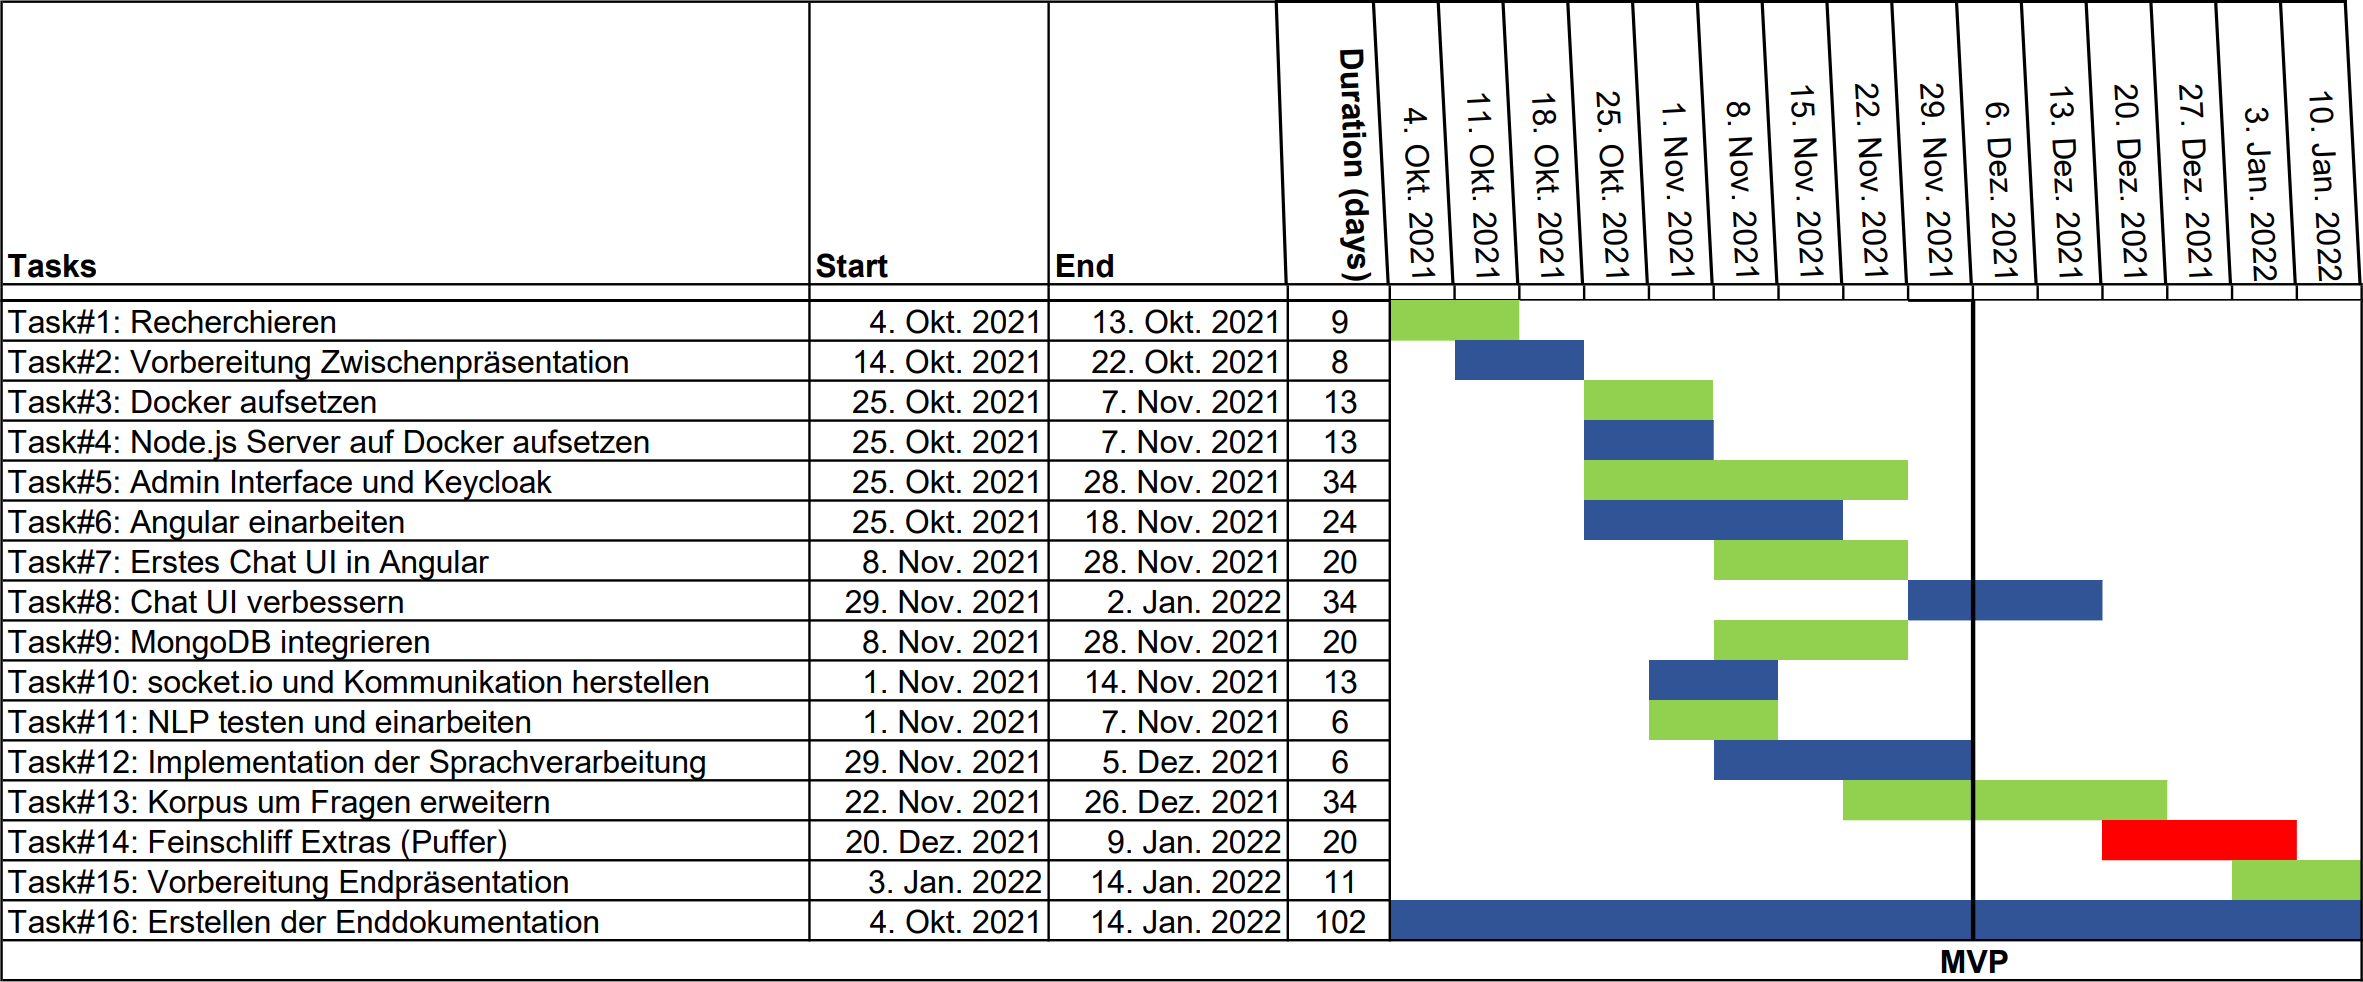
\includegraphics[width=1.0\textwidth]{bilder/zeitmanagement/gantt-diagramm.png}
    \caption{Gantt-Diagramm}
    \label{fig:Gantt-Diagramm}
\end{figure}

\noindent In der Darstellung der Balken stellt eine Spalte, eine Woche dar, beginnend mit jedem Montag.
Am unteren Ende des Diagramms sieht man, wie wir unsere Milestones eingeplant haben.